\begin{figure}
    \begin{center}
    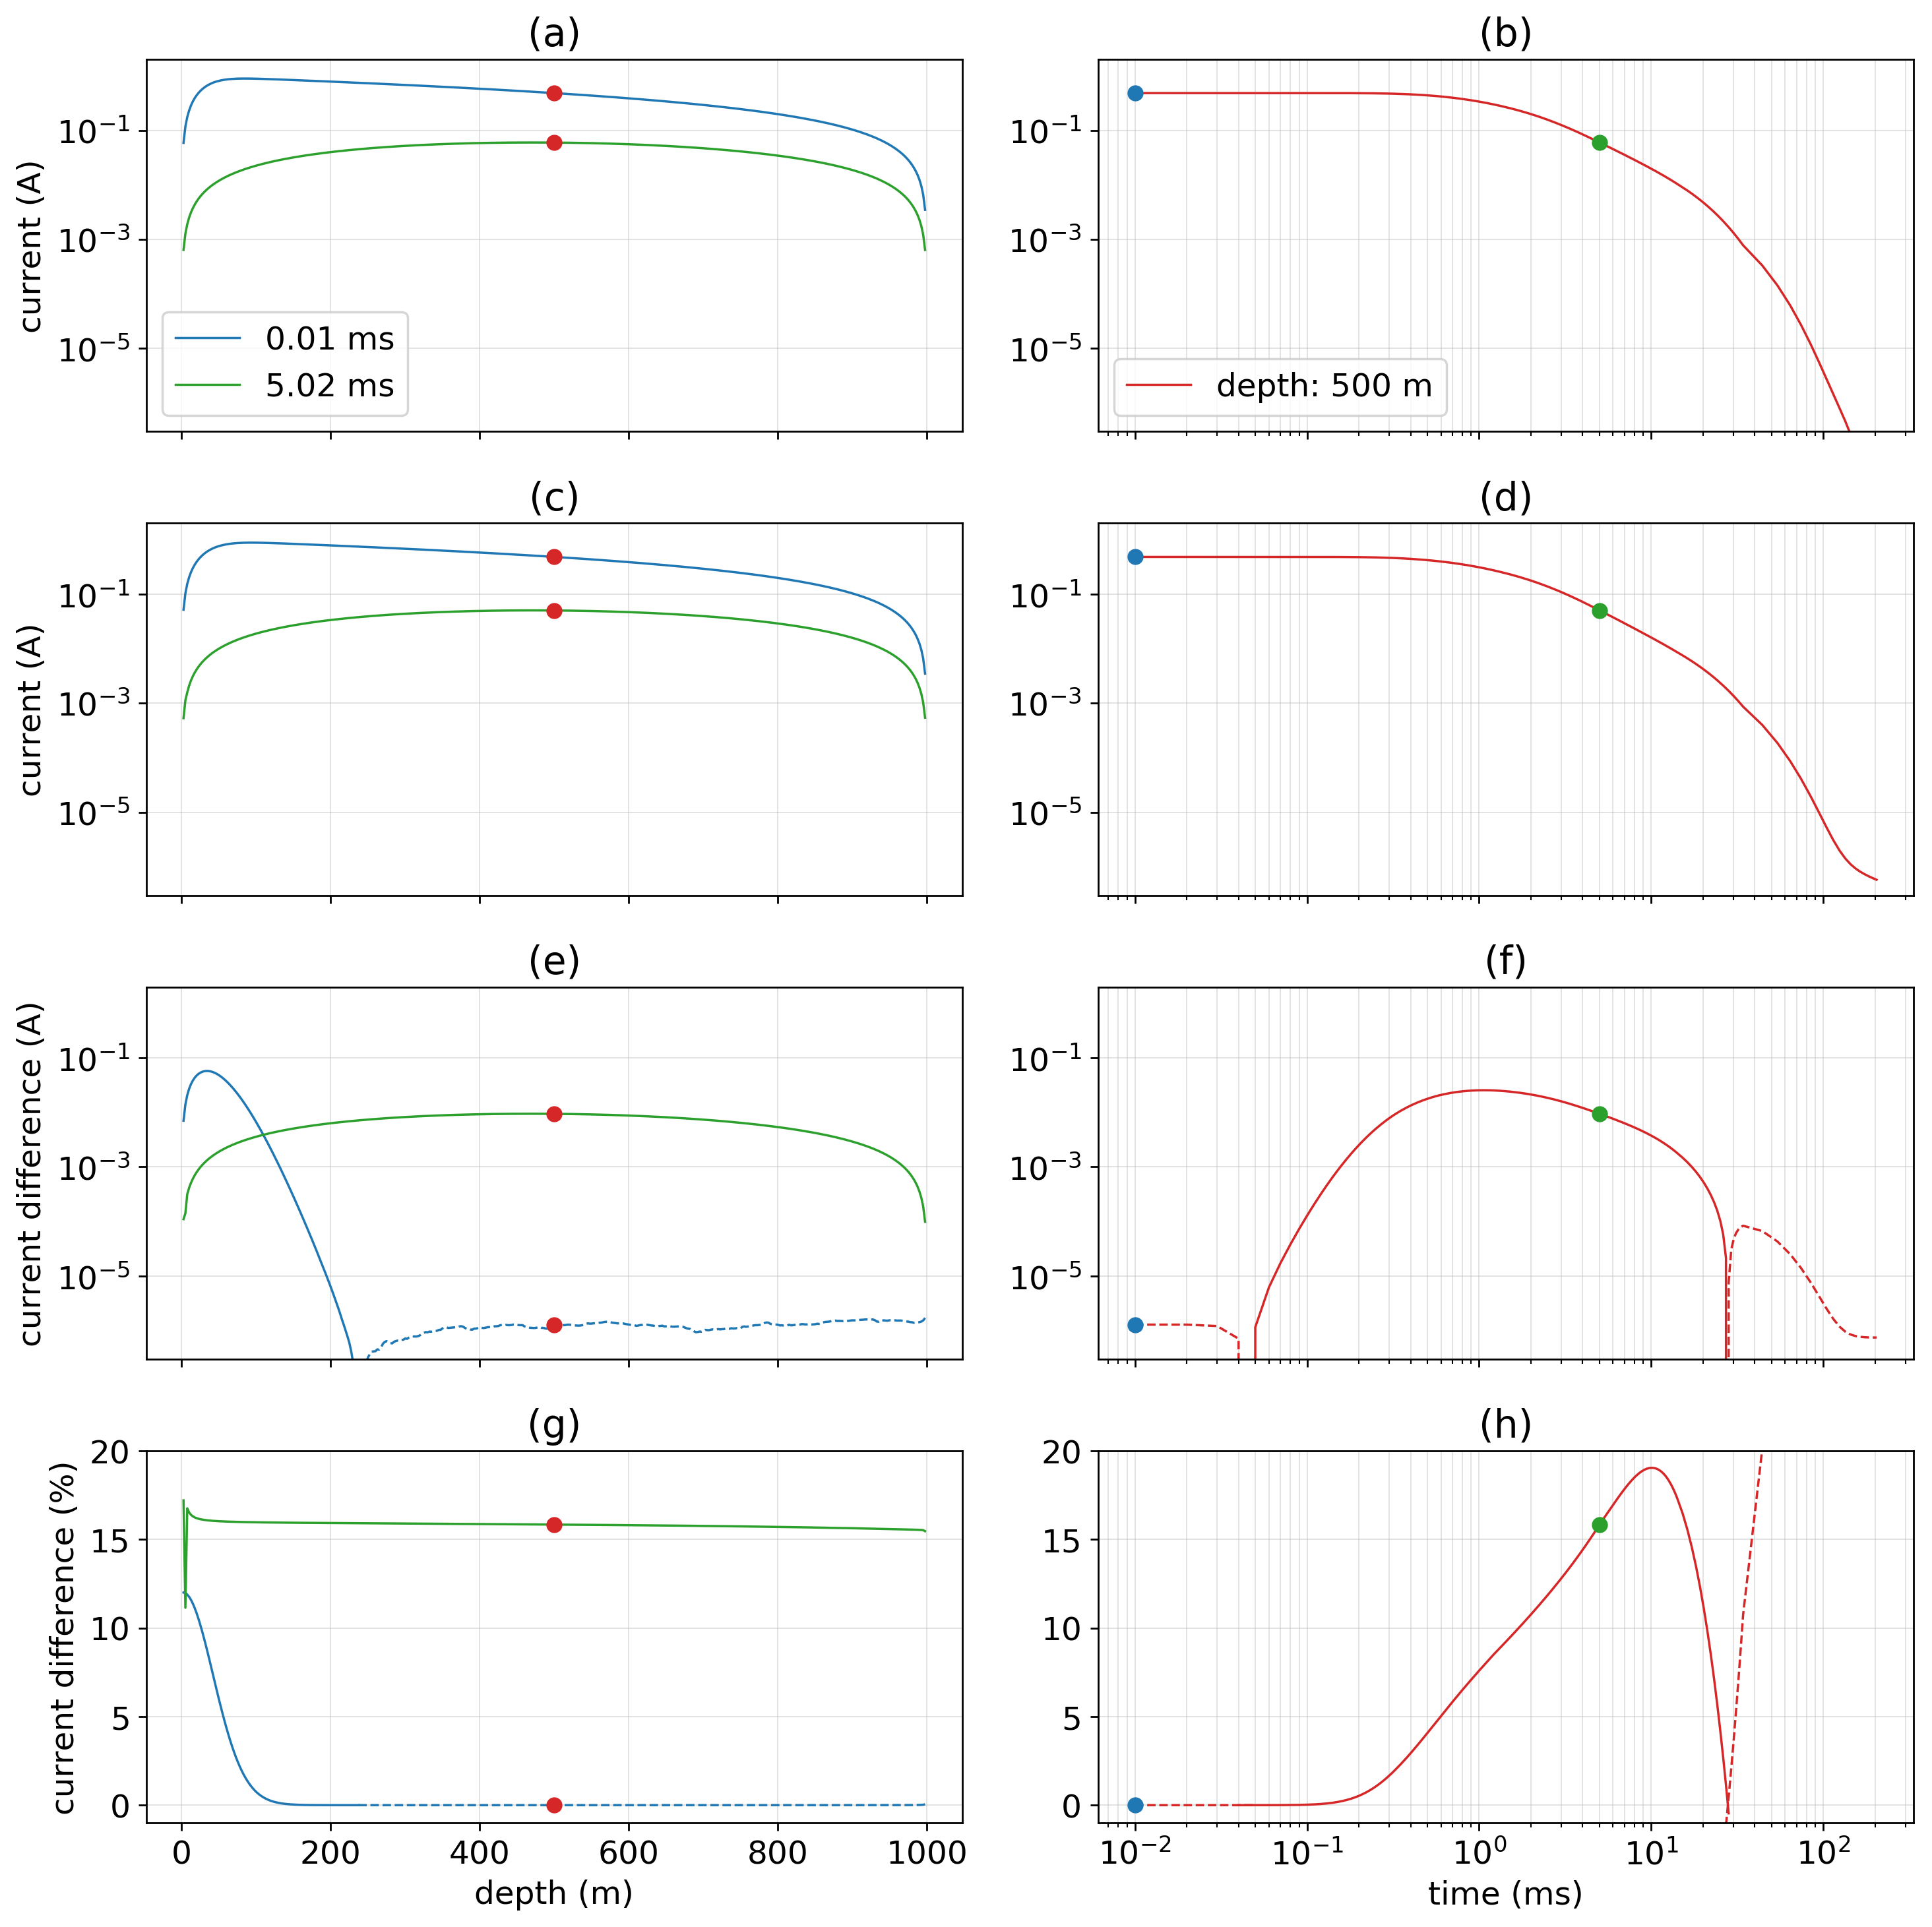
\includegraphics[width=\textwidth]{figures/em_casing/approx_permeable_currents.png}
    \end{center}
\caption{
    (a) Downward-directed current (a) within the casing at 0.01 ms (blue) and 5 ms (green)
    and (b) as a function of time at 500 m depth for the true, permeable, hollow-cased well.
    (c), (d) Current in the approximate model which treats the casing as a solid cylinder.
    The conductivity of the cylinder approximating the well is chosen so that both models have
    equal products of the conductivity and the cross sectional area.
    The permeability of the cylinder is chosen so that both models have equal products of the
    permeability and the thickness.
    (e), (f) Difference between the current in the approximate model and the true model (approximate minus true).
    (g), (h) Difference as a percentage of the true solution.
}
\label{fig:approx_permeable_currents}
\end{figure}



